\documentclass[a4paper, 12pt, openany]{book} %chose the paper size and font size. Openany ensures that all all chapters and similar may begin at any page, not only odd pages. For the introductory pages and appendices we want openany, but for chapter pages in the main content we want chapters to begin only on odd pages (right hand side). The book class ensures that the margins are automatically adjusted such that left hand pages are slightly moved to the left and vice versa at the right, which makes the thesis very readable and good looking when printed in bound book format.

\usepackage[a4paper,top=2cm,bottom=2cm,left=3cm,right=3cm,marginparwidth=1.75cm]{geometry}

\begin{document}

\begin{titlepage}
\newgeometry{left=1.6in, right=2in}
\vspace*{1.5cm}

\noindent  \textcolor{gray}{\large 
Birgitte Louise Vik Thoresen \\ 
Chris Sivert Sylte \\ 
Vegard Arnesen Mytting} \\
\vspace{1cm}

\noindent \textbf{\Large Live Digitization of Chess Games} \\
\vspace{0.5cm}

\noindent {\large Digitization of a chess game based on a camera} \\

\vspace{7cm}
\noindent Bachelor's Thesis in Computer Science \\
Supervisor: Saleh Abdel-Afou Alaliyat \\
May 2025 \\

\vspace{0.2cm}
\noindent Norwegian University of Science and Technology \\
Faculty of Information Technology and Electrical Engineering \\
Department of ICT and Natural Sciences \\

\begin{figure}[h]
    \includegraphics[width=0.28\textwidth]{figures/ntnu_basic.png}
\end{figure}
\end{titlepage}
\restoregeometry
\myemptypage %empty page such that the abstract starts at the first right hand side after the title page

\pagenumbering{roman}

\chapter*{Abstract}
\addcontentsline{toc}{chapter}{Abstract}

% \begin{itemize}
%     \item research question
%     \item methods
%     \item results
%     \item conclusion
% \end{itemize}

The purpose of this project is to develop an automated solution for \aas that enables continuous chess gameplay on a regular board while simultaneously digitizing the game into \gls{pgn} files. The digitized games can be made accessible via an \gls{api} or by streaming moves as events on a message queue. The system leverages image recognition to identify the board and pieces, coupled with real-time validation of moves to ensure compliance with chess rules.\\

The solution is designed to operate on local hardware, typically involving a \acrshort{usb}-connected webcam and a local machine (Windows or Ubuntu), ensuring all processing is performed locally without reliance on cloud infrastructure. While digital chessboards capable of similar functionality exist, they are often costly and require significant setup time for data transmission. This project aims to provide a cost-effective and efficient alternative by automating the digitization process.\\

The development process followed \gls{agile} methodologies, utilizing technologies such as \acrshort{leyolo} and \gls{python} to implement the system. This approach ensured iterative progress, adaptability to changing requirements, and the delivery of a functional and scalable solution.\\

\textbf{*recap of the result is written here*}\\

\textbf{*recap of the conclusion is written here*}

\chapter*{Preface}
\addcontentsline{toc}{chapter}{Preface}

This thesis marks the culmination of our bachelor's degree in Computer Science at NTNU Ålesund, completed during the spring semester of 2025. The project has allowed us to apply our theoretical knowledge to a real-world problem, deepening our understanding of machine learning, software development, and agile workflows. We are grateful for the opportunity to work on a project that combines our interests in chess and software development. \\

We would like to extend our gratitude to our supervisor, \textbf{\saleh}, for his guidance and insightful feedback throughout the duration of this project. We are also thankful to the product owner, \textbf{\arne}, for providing us with the opportunity to undertake this project and for his constructive feedback. Additionally, we would like to acknowledge the external assistance provided by \textbf{\peter}, who supplied the trained model and offered insightful guidance on its structure and practical application.

%%%%%%%%%%%%%%%%%%%%%%%%% TOC %%%%%%%%%%%%%%%%%%%%%%%%%
\newpage

\addcontentsline{toc}{chapter}{Contents}

\tableofcontents

% \newpage

% \newpage

\listoffigures

\newpage

\listoftables

\newpage

\listofcode

\printglossary[type=\acronymtype]

\printglossary

\newpage
%%%%%%%%%%%%%%%%%%%%%%%%%%%%%%%%%%%%%%%%%%%%%%%%%%%%%%%

\pagenumbering{arabic}

\chapter{Introduction}

\section{Background}

Established in 1913, \aas has maintained a longstanding passion for the noble game of chess \cite{schaklag:63}. Over the years, the organization has sought innovative ways to enhance the experience of its members while preserving the integrity and tradition of the game. One of their key objectives is to digitize the process of playing and documenting chess games. Specifically, they aim to develop a cost-effective and user-friendly solution that allows players to engage in continuous gameplay on a traditional chessboard while automatically digitizing the moves into \gls{pgn} files. \cite{ntnuopen:21} This digitization process would enable efficient documentation of games and facilitate advanced analysis using tools such as \gls{stockfish}. By automating the conversion of physical gameplay into digital formats, the organization hopes to eliminate the need for expensive digital chessboards, which often require complex setup procedures.

\section{Project Goal}

The primary objective of this project is to develop a desktop application capable of automating the digitization of chess games played on a traditional board. The application will leverage computer vision and image recognition technologies to capture and interpret gameplay in real-time using a standard webcam connected to a local machine. Key functionalities of the application include:

\begin{itemize}
    \item \textbf{Automatic Digitization:} The application will generate \gls{pgn} files from the captured gameplay, enabling efficient documentation and archival of chess games.

    \item \textbf{Real-Time Visualization:} A digital chessboard will be displayed within the application, updating dynamically to reflect the moves detected by the webcam.

    \item \textbf{Move Analysis:} By generating \gls{fen} strings, the application will integrate with the \gls{stockfish} \gls{api} to provide analysis of gameplay, including suggestions for optimal moves.
\end{itemize}

% This application aims to replicate the functionality of expensive digital chessboards while offering a more cost-effective and accessible alternative. By processing all data locally, the application ensures privacy and eliminates the need for cloud-based infrastructure, making it suitable for use in various settings.

\section{Product Requirements}

The product requirements, as defined by the product owner, outline the essential features and constraints for the proposed solution:

\begin{itemize}
    \item \textbf{Application:} The solution must be implemented as a local application, ensuring compatibility with local machines running either Windows or Ubuntu operating systems.

    \item \textbf{Webcam-Based Detection:} The application must utilize a standard webcam to detect the chessboard, pieces, and moves in real-time.

    \item \textbf{Local Processing:} All data processing, including image recognition and move validation, must be performed locally on the user's machine. Cloud-based solutions are explicitly excluded.

    \item \textbf{Output Formats:} The application must generate \gls{pgn} files for game documentation and \gls{fen} strings to enable integration with the \gls{stockfish} \gls{api} for move analysis.
\end{itemize}

\section{Structure of the Thesis}

\begin{itemize}
    \item \textbf{Chapter 1 -- Introduction:} This chapter introduces the background and motivation for the project, outlines the primary objectives, and defines the product requirements. It establishes the context for the research and development efforts undertaken in this thesis.
    
    \item \textbf{Chapter 2 -- Theory:} This chapter delves into the theoretical foundations of the technologies and methodologies employed in the project. It covers key concepts such as computer vision, image recognition, and the integration of chess analysis tools like \gls{stockfish}.
    
    \item \textbf{Chapter 3 -- Method:} Here, the development process and methodologies are described in detail. This includes the design and implementation of the desktop application, the selection of tools and frameworks, and the approach to solving the problem.
    
    \item \textbf{Chapter 4 -- Results:} This chapter presents the outcomes of the project, including the functionality and performance of the developed application. It highlights the achieved results in relation to the project goals and requirements.
    
    \item \textbf{Chapter 5 -- Discussion:} The results are critically analyzed and discussed in this chapter. It explores the implications of the findings, identifies limitations, and suggests potential areas for future improvement.
    
    \item \textbf{Chapter 6 -- Conclusion:} The final chapter summarizes the project, revisits the objectives, and reflects on the overall success of the solution. It also provides concluding remarks and discusses the broader impact of the work.
\end{itemize}





%%%%% Examples on Code and Figure

% \begin{code}
%     \centering
%     \lstinputlisting[language=python,
%     firstline=1,
%     lastline=5]{code/example.py}
%     \caption{A \gls{python} code}
%     \label{code:python}
% \end{code}

% \begin{figure}
%     \centering
%     \includegraphics[width=0.5\linewidth]{figures/ntnu_basic.png}
%     \caption{Some caption}
%     \label{fig:enter-label}
% \end{figure}

\chapter{Theory}

\section{Literature Review}

The game of chess originated in India during the Gupta dynasty in the 6th century. Over 1500 years later, chess has become a globally recognized game, played competitively in 172 countries worldwide \cite{artsnculture}. \\

With the advancement of technology, various digital solutions and applications have emerged to enhance the experience of playing and analyzing chess. Prominent online platforms such as \textit{Chess.com} and \textit{Lichess.org} allow players to compete across the globe, offering features such as online matchmaking, tutorials, and game analysis. Additionally, physical chessboards have been modernized through the integration of digital technologies, such as \gls{nfc} chips, which enable the digitization of physical chess games. \\

Furthermore, advancements in \gls{ai} have led to the development of applications capable of automating tasks such as piece recognition and game digitization. One notable example is \textit{ChessCam}, a web- and mobile-based application designed for quick and efficient live chess digitization. ChessCam allows users to either upload pre-recorded videos of chess games or stream live games using a mobile phone or webcam. The application processes the video input, recognizes the moves, and generates \gls{pgn} files, which can be used for further analysis or archival purposes.


% \section{Project Management}
% \subsection{Sprint}
% \subsection{Issues}
% \subsection{Meetings}

% \section{Tools and Technologies}
% \subsection{Version Control}

% \section{Design}
% \subsection{UX Design}
% \subsection{Wireframes}

% \section{Code Quality Assurance}
% \subsection{Testing}
% \subsection{Code Review}
% \subsection{Cohesion and Coupling}
% \subsection{Documentation}

\chapter{Methods}
\label{chp:methods}


%% Vi kan sikkert skrive litt om dette i metode

% \subsection{Version Control}
% \label{subsec:version-control}

% The use of \gls{git} as a version control system enables collaborative development by allowing multiple developers to work on the same codebase simultaneously. \gls{git} facilitates the maintenance of the code and provides a comprehensive history of all modifications made to the project. These changes are tracked within project containers known as \glspl{repository}, ensuring transparency and accountability throughout the development process. \cite{alphaefficiency:git}

% \subsubsection*{Branches}

% Git utilizes branches, which are independent lines of development within a repository. Branches allow developers to work on new features, fixes, or experiments without affecting the main codebase. Once changes in a branch are tested and finalized, they can be merged back into the main branch, ensuring a streamlined and controlled integration process. Branching supports parallel development and helps prevent conflicts by isolating work until it's ready for review and integration. \cite{git:branches}

\begin{center}
    \textit{Here, the development process and methodologies are described in detail. This includes the design and implementation of the desktop application, the selection of tools and frameworks, and the approach to solving the problem.}
\end{center}



\section{Machine Learning Models}
\label{sec:ml-models}

After conducting research into existing chess digitization methods, a publicly available solution developed by Peter Batchelor, Tom Richardson, and other contributors was discovered. This solution served as the foundation for the approach. It utilized two \glspl{cnn}: one for detecting chess pieces and another for locating the squares of the chessboard \cite{lichess:chesscam}. \\

Although the documentation for the models was limited, the necessary logic and structure of the models were already present in the repository itself. When additional clarifications were needed, they were obtained through direct communication with the original developers, ensuring that the intended use and functionality of the models were correctly understood. \\

The ChessCam repository provided multiple model formats, including PyTorch and ONNX. Before the models could be used, it was necessary to understand their expected inputs and outputs. Netron was employed to inspect the ONNX files and determine these details. \\

\newpage


\subsection{Piece Detection Model}
The piece detection model was responsible for identifying and classifying chess pieces on the board. It expected \textbf{input} in the format \textbf{[1, 3, 288, 480]}. \textbf{1} represented the batch size, i.e. the number of images processed at once, which was typically set to 1 during inference. \textbf{3} corresponded to the number of color channels (RGB), indicating that the image had to be in color. \textbf{288} and \textbf{480} denoted the height and width of the image in pixels, respectively. \\

The piece model output data in the format \textbf{[1, 16, 2835]}. \textbf{1} represented the batch size. \textbf{2835} represented the number of anchor boxes used in the detection. \textbf{16} consisted of two parts: \\

The first 4 values were offset values that adjusted the position and size of each anchor box to better align with a detected piece. These offsets were relative to the predefined anchor boxes, as illustrated in Table \ref{tab:piece-offset-table}.

\begin{table}[h]
    \centering
    \caption{Offset coordinates for each anchor box with regard to identifying chess pieces.}  % Caption moved to top
    \renewcommand{\arraystretch}{1.5} % Increase row height to allow text to be on top
    \begin{tabular}{lcccc}
        \toprule
        \textbf{Anchor box} & \textbf{xcenter} & \textbf{ycenter} & \textbf{width} & \textbf{height} \\
        \midrule
        Anchor box 1 & -3.23 & 0.57 & -0.12 & -0.34 \\
        Anchor box 2 & 0.51 & -0.63 & 4.15 & 1.27 \\
        Anchor box 3 & 7.71 & 0.29 & -0.11 & 2.45 \\
        ... & ... & ... & ... & ... \\
        Anchor box 2835 & -0.04 & 2.11 & 1.15 & 5.32 \\
        \bottomrule
    \end{tabular}
    \label{tab:piece-offset-table}
\end{table}


The remaining 12 values represented the probabilities for each possible piece type after the offset value had been applied. With 12 different piece types, the model output 12 probabilities for each anchor box. The classification labels are shown in Table \ref{tab:piece-label-table}. Table \ref{tab:piece-probability-table} presents the predicted probabilities for each label across all anchor boxes. \\

\begin{table}[ht]
\centering
\caption{Classification labels for the 12 chess piece types predicted by the model.}
\begin{tabular}{|c|c|}
\hline
\multicolumn{2}{|c|}{\textbf{Model Labels}} \\  % Adds a row at the top
\hline
\textbf{Black Pawn} & \textbf{White Pawn} \\
\textbf{Black Knight} & \textbf{White Knight} \\
\textbf{Black Bishop} & \textbf{White Bishop} \\
\textbf{Black Rook} & \textbf{White Rook} \\
\textbf{Black Queen} & \textbf{White Queen} \\
\textbf{Black King} & \textbf{White King} \\
\hline
\end{tabular}
\label{tab:piece-label-table}
\end{table} 

\\


\begin{table}[h]
    \centering
    \caption{Predicted class probabilities for each anchor box after applying the offsets.}  % Caption moved to top
    \renewcommand{\arraystretch}{1.5} % Increase row height to allow text to be on top
    \begin{tabular}{lcccc}
        \toprule
        \textbf{Anchor box} & \textbf{Black Pawn} & \textbf{White Pawn} & \textbf{Black Knight} & \textbf{...} \\
        \midrule
        Anchor box 1 & \raggedright 0.03 & \raggedright 0.71 & \raggedright 0.01 & ... \\
        Anchor box 2 & \raggedright 0.82 & \raggedright 0.02 & \raggedright 0.01 & ... \\
        Anchor box 3 & \raggedright 0.02 & \raggedright 0.01 & \raggedright 0.78 & ... \\
        ... & ... & ... & ... & ... \\
        Anchor box 2835 & \raggedright 0.01 & \raggedright 0.03 & \raggedright 0.05 & ... \\
        \bottomrule
    \end{tabular}
    \label{tab:piece-probability-table}
\end{table}

\newpage

To summarize, there were 2835 predefined anchor boxes spread across the image, each serving as a candidate location for detecting a chess piece. During training, the model learned to adjust these anchor boxes to better match the actual pieces on the board. It achieved this by predicting 4 offset values that modified the location and size of each anchor box. At runtime, for each anchor box, the model used these learned offsets and output 12 class probabilities, indicating the likelihood of each chess piece type being present at that location.

\newpage

\subsection{Corner Detection Model}
The corner detection model identified the points where the edges of the inner squares on the chessboard met, commonly referred to as intersection points. Up to 49 intersection points could be detected in a single image. These points are illustrated in Figure \ref{fig:xcorners-chessboard}.

\begin{figure}[h!]
    \centering
    \includegraphics[width=0.75\linewidth]{figures/methods/ml-models/xcorners_chessboard.jpg}
    \caption[s]{Visualization of intersection points where the edges of the inner squares on the chessboard meet. The model identified and predicted these points. Up to 49 intersection points could be detected in a single image. \cite{vectorstock:chessboard-svg}}
    \label{fig:xcorners-chessboard}
\end{figure}

The input format for the corner model was the same as the piece model: \textbf{[1, 3, 288, 480]}. The corner model output predictions in the format \textbf{[1, 5, 2835]}. \textbf{1} represented the batch size. \textbf{2835} represented the number of anchor boxes used in the detection. \textbf{5} consisted of two parts: \\

The first \textbf{4 values} were offset values that adjusted the position and size of each anchor box, aligning it more accurately with a potential intersection point. These offsets were relative to the original anchor box coordinates, as shown in Table \ref{tab:corner-offset-table}.

\newpage

\begin{table}[h]
    \centering
    \caption{Offset coordinates for each anchor box with regard to identifying intersection points.}  % Caption moved to top
    \renewcommand{\arraystretch}{1.5} % Increase row height to allow text to be on top
    \begin{tabular}{lcccc}
        \toprule
        \textbf{Anchor box} & \textbf{xcenter} & \textbf{ycenter} & \textbf{width} & \textbf{height} \\
        \midrule
        Anchor box 1 & -1.43 & 3.27 & -0.52 & -2.21 \\
        Anchor box 2 & 2.51 & -7.61 & 0.15 & 4.17 \\
        Anchor box 3 & -3.71 & 1.49 & -4.21 & 2.45 \\
        ... & ... & ... & ... & ... \\
        Anchor box 2835 & -2.04 & 3.29 & -0.35 & 1.24 \\
        \bottomrule
    \end{tabular}
    \label{tab:corner-offset-table}
\end{table}

The final value was the probability that the adjusted anchor box corresponded to an intersection point on the chessboard, as illustrated in Table~\ref{tab:corner-probability-table}. \\

\begin{table}[h]
    \centering
    \caption{Predicted intersection probabilities for each anchor box after applying the predicted offsets.}
    \renewcommand{\arraystretch}{1.5}
    \begin{tabular}{lc}
        \toprule
        \textbf{Anchor Box} & \textbf{Intersection Probability} \\
        \midrule
        Anchor Box 1 & 0.06 \\
        Anchor Box 2 & 0.91 \\
        Anchor Box 3 & 0.03 \\
        ... & ... \\
        Anchor Box 2835 & 0.87 \\
        \bottomrule
    \end{tabular}
    \label{tab:corner-probability-table}
\end{table}


\newpage


\subsection{Combining the models}

To track chess piece movements, the first step was to identify the individual squares of the chessboard. Once the squares were identified, each detected piece needed to be mapped to its corresponding square. This required determining the outer corners of the chessboard. With the corners identified, the board was divided into an 8x8 grid of equally sized squares. Since the distance between the corners was known and all squares in the grid are of uniform size, the centers of the squares could be precisely calculated. For each square, only the center point would be used for subsequent mapping, as shown in Figure~\ref{fig:chessboard-centers}.



\begin{figure}[h!]
    \centering
    \includegraphics[width=0.75\linewidth]{figures/methods/ml-models/outer_corners_centers_chessboard.jpg}
    \caption[S]{Visualization of the outer corners of the chessboard and the centers of each individual square, forming an 8x8 grid. \cite{vectorstock:chessboard-svg}}
    \label{fig:chessboard-centers}
\end{figure}


The bottom center of each piece’s bounding box was selected as its representative location, as highlighted in Figure~\ref{fig:bbox-black-pawn}. Each detected piece was then mapped to the nearest square center based on the minimum euclidean distance. This mapping allowed for the precise determination of each piece's position on the chessboard.



\newpage

\begin{figure}[h!]
    \centering
    \includegraphics[width=0.25\linewidth]{figures/methods/ml-models/black-pawn.png}
    \caption[FIX]{Example of a detected chess piece with its classification confidence. The bottom center of the bounding box was used as the reference point for mapping the piece to its corresponding square. \cite{svgrepo:black-pawn-svg}}
    \label{fig:bbox-black-pawn}
\end{figure}

\subsubsection*{Implementation}

THIS IS Not finished

The piece detection model is responsible for identifying and classifying chess pieces. It expected an input image of size 288x480 with three color channels. Since video frames typically do not come in this exact format, the images are first scaled to the required dimensions to ensure compatibility with the model.

To identify candidate quadrilaterals on the chessboard, the implementation first performs Delaunay triangulation over the set of detected corner points. It then searches for pairs of adjacent triangles—triangles that share two vertices—and combines their points to form four-point quads. This method restricts the candidates to geometrically relevant regions made up of neighboring points, avoiding the need to evaluate all possible 4-point combinations, which would be computationally expensive and less accurate.



The reason for doing it this way, is that unlike detecting the 4 corners of the board directly, the algorithm can still run successfully even if various parts of the board are obscured. The question then becomes, how does it find the corners from these points?


There are in total 12 class labels each for the type piece and which color it is.

After processing the image, the model returns a set of predictions for each potential piece. These predictions include:

The model predicts these values for each anchor box. An anchor box is a predefined bounding box within the image that serves as a potential candidate location for a piece. By adjusting these anchor boxes, the model can detect and classify pieces across different positions on the chessboard.

\begin{subfigure}[h!]{0.9\linewidth} \centering \includegraphics[width=\linewidth]{figures/methods/ml-models/piece-model.png} \caption{Tournament View} \end{subfigure}

\newpage


\section{Agile Methodology}
\label{sec:development-methodology}

The team organized their work into bi-weekly \textbf{sprints}, each culminating in a status report and retrospective. At the beginning of each sprint, the product backlog was reviewed to prioritize tasks for the upcoming sprint. Sprint goals were then set, and each team member outlined the tasks they planned to complete before the next meeting. The team reviewed completed tasks to assess progress. For any incomplete tasks, potential causes were discussed, and strategies for addressing them were devised. At the end of each sprint, retrospectives provided an opportunity for the team to reflect on their collaboration and identify areas for improvement. \\

To manage and track tasks, the team utilized GitHub’s \textbf{Issue Board}. Issues were categorized as follows: \textit{Enhancement} for new features or improvements, \textit{Documentation} for adding explanations or improving code safety, \textit{Bug} for errors or unexpected behaviors, and \textit{Task} for general tasks. Each issue was assigned to one or more team members to clarify responsibilities. The Issue Board was organized into four columns: \textit{No Status}, \textit{To Do}, \textit{In Progress}, and \textit{Done}, providing a clear visual overview of progress. \\

For \textbf{code review}, the team used GitHub pull requests. Each issue was worked on in a separate branch, enabling team members to review and discuss contributions before merging them into the main codebase.


% Jeg kommenterer disse ut ettersom jeg ikke helt vet hva som er ønsket skal stå under disse
%\subsubsection*{Product Owner}

%\subsubsection*{Supervisor}


\section{Architecture}
\label{subsec:diagrams}

To provide a comprehensive understanding of the system architecture and interaction flow, several \gls{uml} diagrams were created. These diagrams model different aspects of the live chess game digitization system, from component interactions and activity flow to user roles and use cases.

\subsubsection*{Sequence Diagram}
\label{subsubsec:sequence-diagram}

The sequence diagram, shown in Figure \ref{fig:sequence}, illustrates the chronological flow of interactions between the system components and external actors. It begins with the Admin initiating the game recording by setting up the camera, which captures and streams the board state to a local processing unit. This unit continuously detects and validates moves, updating the user interface accordingly. Users, from remote devices, can spectate the game in real time or save it as a \gls{pgn} file. The diagram emphasizes the communication between hardware (camera and local machine) and the \gls{ui}, highlighting how physical chess games are digitized and broadcasted.

\newpage

\begin{figure}[h!]
    \centering
    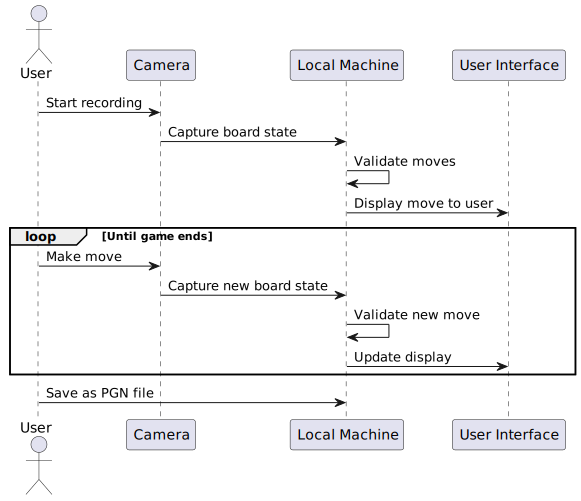
\includegraphics[width=0.75\linewidth]{figures/methods/uml/sequence.png}
    \caption[Sequence Diagram]{Sequence Diagram}
    \label{fig:sequence}
\end{figure}

\subsubsection*{Use-Case Diagram}
\label{subsubsec:use-case-diagram}

The use-case diagram, shown in Figure \ref{fig:use-case}, identifies the system’s main actors and the primary functionalities they interact with. Admins are responsible for hardware setup and initiating the game recording process. The system autonomously handles move detection, validation, and \gls{ui} updates. Users, on the other hand, access the game remotely to spectate or download \gls{pgn} files. This diagram provides a clear overview of who interacts with the system and what capabilities are exposed, forming the basis for understanding system requirements and user expectations.

\begin{figure}[h!]
    \centering
    \includegraphics[width=0.75\linewidth]{figures/methods/uml/use-case.png}
    \caption{Use-Case Diagram}
    \label{fig:use-case}
\end{figure}

\begin{figure}[h!]
    \subsubsection*{Activity Diagram}
    \label{subsubsec:activity-diagram}
    
    \centering
    \begin{minipage}[t]{0.5\textwidth}
        \vspace{0pt}
        The activity diagram, shown in Figure \ref{fig:activity}, provides a high-level overview of the operational workflow during a chess game session. It models the continuous loop of capturing board states, detecting and validating moves, and updating the game state until the game ends. If a move is invalid, the system flags it but does not terminate the session. Once the game concludes, it is converted into a standard \gls{pgn} format. This diagram emphasizes the logical flow and decision-making process, reflecting the system’s role in automating and maintaining the integrity of live digitization.
    \end{minipage}
    \hfill
    \begin{minipage}[t]{0.45\textwidth}
        \vspace{0pt}
        \includegraphics[width=\linewidth]{figures/methods/uml/activity-2.png}
        \caption[Activity Diagram]{Activity Diagram}
        \label{fig:activity}
    \end{minipage}
\end{figure}

\subsection{Wireframes}
\label{subsec:wireframe}

\subsubsection*{Control Panel}

The Control Panel is a desktop interface for tournament organizers to manage the digitization of multiple physical chess boards. It follows a simple three-step workflow:

\begin{enumerate}
\item \textbf{Select Number of Cameras:} Specify the number of boards to monitor, which determines how many camera feeds are initialized (Figure \ref{fig:control-panel-1}).
\item \textbf{Start Cameras and Digitization:} Launches the camera feeds, board state recognition, and move validation (Figure \ref{fig:control-panel-2}).
\item \textbf{Restart Boards for New Round:} Resets all boards at the end of a round, preparing the system for the next games (Figure \ref{fig:control-panel-3}).
\end{enumerate}

The interface is minimal and task-focused, enabling efficient system setup and management with little technical effort.

\begin{figure}[h!]
    \centering
    \begin{subfigure}[h!]{0.40\linewidth}
        \centering
        \includegraphics[width=\linewidth]{figures/methods/wireframes/control-panel-1.png}
        \caption{Step 1}
        \label{fig:control-panel-1}
    \end{subfigure}
    \hfill
    \begin{subfigure}[h!]{0.40\linewidth}
        \centering
        \includegraphics[width=\linewidth]{figures/methods/wireframes/control-panel-2.png}
        \caption{Step 2}
        \label{fig:control-panel-2}
    \end{subfigure}

    \begin{subfigure}[h!]{0.40\linewidth}
        \centering
        \includegraphics[width=\linewidth]{figures/methods/wireframes/control-panel-3.png}
        \caption{Step 3}
        \label{fig:control-panel-3}
    \end{subfigure}
    
    \caption{Control Panel wireframes showing sequential interaction steps}
    \label{fig:control-panel-group}
\end{figure}


\begin{figure}[h!]
\subsubsection*{Desktop View}
    \centering
    \begin{subfigure}[h!]{0.40\linewidth}
        \centering
        \includegraphics[width=\linewidth]{figures/methods/wireframes/desktop-tournament-view.png}
        \caption{Tournament View}
        \label{fig:desktoop-tournament-view}
    \end{subfigure}
    \hfill
    \begin{subfigure}[h!]{0.40\linewidth}
        \centering
        \includegraphics[width=\linewidth]{figures/methods/wireframes/desktop-board-view.png}
        \caption{Board View}
        \label{fig:desktop-board-view}
    \end{subfigure}

    \begin{subfigure}[h!]{0.40\linewidth}
        \centering
        \includegraphics[width=\linewidth]{figures/methods/wireframes/desktop-full-screen-video-view.png}
        \caption{Fullscreen Video Feed}
        \label{fig:desktop-fullscreen-video}
    \end{subfigure}
    
    \caption{Desktop client-side view wireframes}
    \label{fig:desktop-view-group}
\end{figure}

\begin{figure}[h!]
\subsubsection*{Phone View}
    \centering
    \begin{subfigure}[h!]{0.2\linewidth}
        \centering
        \includegraphics[width=\linewidth]{figures/methods/wireframes/phone-tournament-view.png}
        \caption{Tournament View}
        \label{fig:phone-tournament-view}
    \end{subfigure}
    \hfill
    \begin{subfigure}[h!]{0.2\linewidth}
        \centering
        \includegraphics[width=\linewidth]{figures/methods/wireframes/phone-board-view.png}
        \caption{Board View}
        \label{fig:phone-board-view}
    \end{subfigure}
    \hfill
    \begin{subfigure}[h!]{0.2\linewidth}
        \centering
        \includegraphics[width=\linewidth]{figures/methods/wireframes/phone-full-screen-video-view-vertical.png}
        \caption{Vertical Fullscreen Video Feed}
        \label{fig:phone-fullscreen-video-vertical}
    \end{subfigure}
    \hfill
    \begin{subfigure}[h!]{0.2\linewidth}
        \centering
        \includegraphics[width=\linewidth]{figures/methods/wireframes/phone-full-screen-video-view-horizontal.png}
        \caption{Horizontal Fullscreen Video Feed}
        \label{fig:phone-fullscreen-video-horizontal}
    \end{subfigure}
    
    \caption{Phone client-side view wireframes}
    \label{fig:phone-view-group}
\end{figure}

\section{Tools and Platforms}
\label{sec:tools-and-platforms}

\subsection*{Development Tools}
\label{subsec:development-tools}

\begin{itemize}
    \item \textbf{\gls{vscode}} was used as the primary development environment due to its support for multiple programming languages and extensions.
\item \textbf{Postman} was employed for testing and validating RESTful \glspl{api}, utilizing built-in JavaScript-based test snippets.
\item \textbf{Netron.app} was used to visualize neural network architectures during the evaluation phase.
\item \textbf{Git} facilitated version control and collaboration throughout the development process.
\item \textbf{\glspl{llm}} (e.g., ChatGPT) were consulted to review code and provide suggestions, functioning as a collaborative assistant.
\item \textbf{Lighthouse} was used to evaluate and improve the performance and accessibility of the developed web interface.
\end{itemize}.

\subsection*{Collaboration Tools}
\label{subsec:collaboration-and-design-tools}

\begin{itemize}
    \item \textbf{GitHub} was used for its built-in project management tool, which allowed the team to create an Issue Board for easy issue tracking. It was also used for code reviews and version control management.
    
    \item \textbf{Figma} was used as a tool for sketching and creating wireframes.
    
    \item \textbf{OneDrive} was used as a platform for storing and sharing files.
    
    \item \textbf{Overleaf} was used as the platform for writing the report, utilizing its LaTeX support to efficiently compose and format the thesis.
\end{itemize}


\section{Technology Stack}
\label{sec:technology-stack}

\subsection*{Backend}
\subsubsection*{Python libraries}

\begin{itemize}
    \item \textbf{chess} – Used for move generation, validation, and parsing of chess game formats. \cite{python:chess}
    \item \textbf{FastAPI} – Web framework used to develop RESTful APIs for backend services. \cite{python:fastapi}
    \item \textbf{numpy} – Core package for numerical operations. \cite{python:numpy}
    \item \textbf{onnxruntime} Used for running pre-trained machine learning models. \cite{python:onnx}
    \item \textbf{opencv-python} Utilized for computer vision tasks. \cite{python:opencv}
    \item \textbf{requests} – Used to handle HTTP communication. \cite{python:requests}
    \item \textbf{scipy} – Employed for scientific and numerical computations. \cite{python:scipy}
    \item \textbf{tensorflow}, Used to build and execute machine learning models. \cite{python:tensorflow}
\end{itemize}


\subsection*{Frontend}
\subsubsection*{TypeScript libraries}

\begin{itemize}
    \item \textbf{Vite} is a fast frontend build tool of web applications. \cite{ts:vite}
    
    \item \textbf{React} builds user interfaces out of individual pieces called components. \cite{ts:react}
    
    \item \textbf{@vitejs/plugin-react-swc} Speeds up the Vite development server. \cite{ts:swc}
    
    \item \textbf{chess.ts} a Typescript chess library for chess move generation/validation, piece placement/movement, and check/checkmate/draw detection \cite{ts:chess}
    
    \item \textbf{react-dom} serves as the entry point to the DOM and server renderers for React. \cite{ts:react-dom}
\end{itemize}

\section{Testing}
\label{sec:testing}

\subsection{Model testing}
\label{subsec:model-testing}

The performance of the machine learning model was evaluated through 100 test games. Five distinct chess openings were selected, with 10 games played per opening on each of two board types: plastic and wooden. This resulted in 50 games per board type. Each game consisted of 15 full moves, corresponding to 15 moves by white and 15 moves by black. \\

Each move was logged as either successful or unsuccessful. A 30-second window was provided for the model to detect and transmit each move, starting from the moment the move was made \gls{otb}. If the model failed to detect the move within this time frame, or if it detected the wrong move, it was marked as unsuccessful. The game concluded either when a move was marked unsuccessful or all 15 full moves had been completed. \\

The webcam was mounted above the board at an angle of approximately 60–70\si{\degree}
 relative to the table surface. The white pieces were placed on the left side of the camera's field of view, and the black pieces on the right.

\begin{figure}[h!]
    \centering
    \includegraphics[width=0.75\linewidth]{figures/methods/testing/setup.png}
    \caption[Setup during testing]{Physical setup during testing, showing the board, webcam position, and piece orientation.}
    \label{fig:setup}
\end{figure}

\newpage



\subsection{Wireframe testing}
\label{subsubsec:user-centered-design}

The following processes align with the principles discussed in  Subsection~\ref{subsec:usability-testing} 
outlined in Chapter~\ref{chp:theory}. At the beginning of the design process, the group conducted wireframe testing with a diverse set of users. This included participants of varying age groups from young to elderly as well as both chess players and non-chess players. The goal was to evaluate whether users found the interface intuitive and whether the sizing and layout were appropriate. \\

All participants were given the same context before starting the test: 

\begin{quote}
\textit{You are viewing a chess game between two companions you know. You visit the tournament organizer's website and come across this webpage.}
\end{quote}

Participants were then either given specific tasks to perform within the application or asked to explore freely, mimicking a real-world scenario. This approach aimed to identify how naturally users could navigate and understand the application without explicit instruction. \\

After completing their interaction with the application, participants filled out an anonymous feedback form. The form included the following questions:

\begin{itemize}
    \item \textit{On a scale from 1 to 5, how satisfied are you with the overall experience of the application?}
    \item \textit{On a scale from 1 to 5, how satisfied are you with the Tournament View page?}
    \item \textit{On a scale from 1 to 5, how satisfied are you with the Board View page?}
    \item \textit{Do you have any feedback, suggestions for improvement, or features you would like to see added?}
\end{itemize}

See Subsection \ref{subsec:wireframe} for the final tested wireframe.

\newpage

\subsection{Color palette testing}
\label{subsubsec:color-palette}

In selecting the application's color palette, the group opted for a variation of blue. This choice was influenced by the symbolic associations of the color blue, which is often linked to imagination, intelligence, and wisdom \cite{blue} traits that are relevant to the game of chess \cite{chess:ppqty, chess:chess-and-creativity}. \\

To identify the most suitable stylistic direction, several versions of the application were developed, each showcasing a distinct color palette. These prototypes were printed and displayed in a shared space, allowing individuals from diverse backgrounds to view and compare them. \\

Participants were invited to vote for their preferred versions via a form. Each participant was allowed up to three votes and had the option to leave comments. For instance, some expressed a preference for the light mode from palette \#08 and the dark mode from palette \#07, while others favored the board design from palette \#05 or the move-highlighting style from palette \#14. \\

Rather than selecting a single predefined palette, the final color scheme was assembled by combining the most highly rated elements across the top-voted variations. This approach allowed for a more tailored and user-informed visual design (See Figure \ref{fig:color-palette-results} for the vote results). \\

\begin{figure}[h!]
    \centering
    \includegraphics[width=0.75\linewidth]{figures/methods/color-palette-results.png}
    \caption{Distribution of Votes Across Different Color Palettes}
    \label{fig:color-palette-results}
\end{figure}

See Appendix~\ref{app:color-palettes} for the full set of tested color palettes.

\chapter{Results}


\begin{center}
    \textit{This chapter presents the outcomes of the project, including the functionality and performance of the developed application. It highlights the achieved results in relation to the project goals and requirements.}
\end{center}

\section{Machine Learning Model}

The performance of the machine learning model was evaluated through 100 test games. Five distinct chess openings were tested, with 10 games per opening on each of two board types: plastic and wooden. This resulted in 50 games per board type. Each game consisted of 15 full moves (15 moves by white and 15 moves by black). \\

Each move was logged as either successful or unsuccessful. A 30-second window was provided for the system to detect and transmit each move, starting from when the move was made over-the-board (OTB). If the system failed to detect the move within this window or detected an incorrect move, it was marked as unsuccessful. The game concluded once a move was marked unsuccessful or all 15 full moves were completed.

\newpage

\begin{table}[htbp]
\centering
\caption{Move detection accuracy on both wooden and plastic boards}
\begin{tabular}{lccc}
\toprule
\textbf{Category} & \textbf{OTB Moves} & \textbf{Successful Moves} & \textbf{Accuracy (\%)} \\
\midrule
\textbf{Total} & 1033 & 936 & 90.6\% \\
\midrule
\textbf{White Pieces} & & & \\
\hspace{1em}Pawn  & 244 & 242 & 99.2\% \\
\hspace{1em}Knight & 128 & 117 & 91.4\% \\
\hspace{1em}Bishop & 74  & 54  & 73.0\% \\
\hspace{1em}Rook   & 29  & 25  & 86.2\% \\
\hspace{1em}Queen  & 42  & 40  & 95.2\% \\
\hspace{1em}King   & 16  & 8   & 50.0\% \\
\midrule
\textbf{Black Pieces} & & & \\
\hspace{1em}Pawn  & 247 & 243 & 98.4\% \\
\hspace{1em}Knight & 78  & 75  & 96.2\% \\
\hspace{1em}Bishop & 65  & 47  & 72.3\% \\
\hspace{1em}Rook   & 21  & 5   & 23.8\% \\
\hspace{1em}Queen  & 84  & 76  & 90.5\% \\
\hspace{1em}King   & 5   & 4   & 80.0\% \\
\bottomrule
\end{tabular}
\end{table}

\begin{table}[htbp]
\centering
\caption{Summary of Total Moves and Success Rate by Board Type}
\begin{tabular}{lccc}
\toprule
\textbf{Board Type} & \textbf{Total Moves} & \textbf{Total Successful Moves} & \textbf{Success Rate (\%)} \\
\midrule
Plastic & 475 & 427 & 89.9\% \\
Wooden  & 558 & 509 & 91.2\% \\
\bottomrule
\end{tabular}
\end{table}


\newpage


\begin{figure}[htbp]
\centering
\begin{tikzpicture}
\begin{axis}[
    ybar,
    bar width=8pt,
    width=\textwidth,
    height=8cm,
    enlarge x limits=0.05,
    ymin=0,
    ylabel={Number of Games Failed},
    xlabel={Move Number},
    xtick={1,...,15,All},
    xticklabels={1,2,3,4,5,6,7,8,9,10,11,12,13,14,15,All},
    x tick label style={rotate=45, anchor=east},
    legend style={at={(0.5,-0.25)}, anchor=north, legend columns=-1},
    nodes near coords,
    symbolic x coords={1,2,3,4,5,6,7,8,9,10,11,12,13,14,15,All},
    xticklabel style={font=\small},
]
\addplot+[style={fill=blue!50}] coordinates {
    (1,0) (2,12) (3,2) (4,10) (5,14) (6,4) (7,3) (8,3) (9,0)
    (10,0) (11,0) (12,0) (13,0) (14,0) (15,0) (Completed All,2)
};
\addplot+[style={fill=red!50}] coordinates {
    (1,0) (2,6) (3,6) (4,16) (5,5) (6,3) (7,1) (8,0) (9,6)
    (10,0) (11,0) (12,1) (13,3) (14,1) (15,0) (All,2)
};
\legend{Plastic, Wooden}
\end{axis}
\end{tikzpicture}
\end{figure}

\begin{table}[htbp]
\centering
\caption{Frequencies of Different Detection Errors}
\begin{tabular}{lccc}
\toprule
\textbf{Board Type} & \textbf{Total Failures} & \textbf{No Detection} & \textbf{Incorrect Detection} \\
\midrule
Plastic & 48 & 47 & 1 \\
Wooden & 48 & 40 & 8 \\
\midrule
\textbf{Total} & 96 & 87 & 9 \\
\bottomrule
\end{tabular}
\end{table}

For a detailed breakdown of the chess games, including the sequences of moves, failure points, and detection statistics for each board type, see Appendix FILL IN.




\section{Overview of Delivered Product}
The delivered product refers to the final version of the application submitted at the conclusion of this Bachelor’s thesis. The application was developed at the request of the product owner and based on the requirements provided. The initial description served as a general concept rather than a detailed specification, which meant that decisions regarding design, architecture, and technology were left to the development team. Throughout the development process, ideas and design choices were discussed with the product owner and approved during regular meetings. \\

The application was developed as an open-source project with the intention that the code can be reused, maintained, and extended by others. All components are built using open and freely available technologies, ensuring that the system can be installed on local hardware without the need for licensed software or cloud-based services. This aligns with the requirement that all processing should be performed locally, using common hardware such as a webcam connected to a local machine running either Windows or Ubuntu. \\

The project follows clear coding standards and development best practices, making the code easy to understand and modify. All functionality is well documented, enabling future developers to build upon the existing solution. For example, to support new chess variants, integrate additional hardware, or improve the recognition models. To support future development and accessibility, the source code is published in a public Git repository without restrictions on reuse or adaptation. \\

The application itself is a local, camera-based system for digitalizing over-the-board chess games in real time. It detects piece movements on a physical chessboard using image recognition and converts the game into a PGN file, which can be viewed or analyzed digitally. The system operates entirely on local hardware, with a front-end interface that allows users to follow games live and a back-end that manages board recognition and game logic. The application is designed to be low-cost, open-source, and easy to maintain, with extensibility in mind for future features.

\section{Functional Results}
The application consists of three main components: machine learning, WebSocket communication, and the front-end interface. The back-end handles image recognition and game logic, using a machine learning model to detect board states. It communicates with the front-end through a WebSocket connection. The front-end is responsible for presenting this information to the user in real time. The cameras is connected with a USB-hub, where multiple cameras can be attached to the same computer. 

\subsection{Machine Learning}
To be completed.

\subsection{API}
To enable real-time updates and improve the responsiveness of the front-end interface, the application uses a WebSocket connection between the back-end and the front-end. This method was suggested by the product owner and was also approved by the supervisor. This communication channel is used for transmitting move data as it is detected by the board recognition system. Unlike traditional HTTP requests, which operate on a request-response basis, WebSocket allows for continuous, two-way communication between the server and the client. \\

Once the application initiates a connection, the WebSocket remains open throughout the session. As new moves are identified on the physical board, the back-end sends the corresponding move data as messages through the WebSocket. These messages are then received by the front-end, which updates the displayed move list and board state in real time. This provides a seamless viewing experience for users following live games. \\

The WebSocket server also handles specific command messages. For example, when the server sends a message labeled "RESET," the front-end clears the current move list, typically indicating the start of a new game. A message labeled "INVALID" is used to signal an unrecognized or incorrect move and does not trigger any front-end changes. All other messages are assumed to be valid algebraic notation representing chess moves and are appended to the game history displayed to the user. \\

The WebSocket functionality is encapsulated in a custom React hook on the front-end, which manages the connection lifecycle and state updates. This abstraction simplifies integration into the user interface and ensures that resources are properly cleaned up when the component is unmounted. Overall, the use of WebSocket communication is a key component in delivering a responsive and live experience, particularly for tournaments and public displays where move-by-move tracking is essential.

\subsection{Frontend}
The front-end of the application serves as the user interface. It includes a control panel for tournament organizers and a web application for spectators. The application's main responsibility is to visualize the chessboard and display ongoing moves. The front-end communicates with the back-end via WebSocket to ensure real-time updates and interactivity. \\

The \textbf{control panel} is an administrative tool accessible only to the tournament organizers. It functions as a standalone dashboard application and is available exclusively on the computer that starts the application, as shown in Figure~\ref{fig:control-panel}. This setup ensures that spectators visiting the website cannot access the control panel. \\

\begin{figure}[h!] \centering \includegraphics[width=0.75\linewidth]{figures/results/frontend/control-panel/control-panel.png} \caption[Control panel for tournament organizers]{The control panel used by the tournament organizers.}\label{fig:control-panel} \end{figure}

Before the tournament begins, the organizer must start the application and configure it using the control panel. This includes specifying the number of cameras to be used, allowing the application to connect to the appropriate number of video feeds. When the number of selected cameras is connecting, a progress bar is visible for the user, as shown in Figure~\ref{fig:control-panel-camera} Once the connections are established, the tournament can be started by pressing the "Start Tournament" button. \\
 
\begin{figure}[h!] \centering \includegraphics[width=0.75\linewidth]{figures/results/frontend/control-panel/camera-progress.png} \caption[Progress bar for camera connections]{A progress bar representing the status of connecting cameras}\label{fig:control-panel-camera} \end{figure}

When completed connecting the cameras successfully, a success message is displayed, as shown in Figure~\ref{fig:control-panel-camera-success}. If the organizer attempts to connect more cameras than the system can detect, an error message is displayed, as shown in Figure~\ref{fig:control-panel-camera-error}. This provides feedback to the user about what went wrong. For example, the message "Error: Could not open Camera 1" indicates that the system could not find a camera with ID 1. In the illustrated scenario, no cameras were connected, which caused the error to appear. \\

\begin{figure}[h!] \centering \includegraphics[width=0.75\linewidth]{figures/results/frontend/control-panel/camera-success.png} \caption[Success message for camera connections]{A success message for  connecting cameras correctly}\label{fig:control-panel-camera-success} \end{figure}

\begin{figure}[h!] \centering \includegraphics[width=0.75\linewidth]{figures/results/frontend/control-panel/camera-error.png} \caption[Error message for camera connections]{A error message for failure connecting cameras}\label{fig:control-panel-camera-error} \end{figure}

The control panel also provides functionality for resetting individual boards or all boards simultaneously. When a tournament round is finished, the organizers must reset all boards before the next round can begin. By pressing the "Reset All Boards" button, they can reset all connected boards at once. In some scenarios, it may be necessary to reset a single board. In such cases, the organizers can use the "Select Which Board to Reset" feature, as shown in Figure~\ref{fig:control-panel-reset-boards}. \\

\begin{figure}[h!] \centering \includegraphics[width=0.75\linewidth]{figures/results/frontend/control-panel/reset-boards.png} \caption[Panel to reset a single board]{The panel to select which board to be reset}\label{fig:control-panel-reset-boards} \end{figure}

The \textbf{web application} was designed for spectators  who want to follow the tournament and watch the games being played. It includes several features that present the tournament in a user-friendly manner. These include a Tournament View, which displays a table of all ongoing games; a Game Preview page with summaries of each game; and a Board View, which shows the chessboard, \gls{pgn} display, and a live camera feed for a specific board. The application also contains a header with links to informational pages such as "How it Works", which explains how to use the system, and "About", which outlines the project’s purpose and requirements. \\

The application is implemented as a \textbf{responsive} web application that functions on both desktop and mobile devices. The layout adapts to different screen sizes, which helps maintain usability across platforms. Key interface elements such as navigation, buttons, and forms adjust to fit smaller screens, making it possible to use the application on smartphones and tablets as well. It also includes an option to switch between light and dark color modes. This setting can be changed in the system preferences and allows users to choose the visual style they find more comfortable. The color palettes are adjusted accordingly, providing a consistent appearance throughout the interface depending on the selected mode. \\

For demonstration purposes, a \textbf{dataset} of chess players was created and displayed in the Tournament View. This dataset includes real professional chess players along with their corresponding ratings, in order to simulate multiple boards and games. Since the available hardware for testing was limited to only two cameras, a mocked dataset was used to represent additional boards and players during the demonstration. \\

When the application is started, both the control panel and the web application launch simultaneously. This means the web application is accessible even before the tournament has officially started. Upon entering the web application, the initial page shown is the \textbf{Tournament View}. If the tournament has not yet started, this view contains no data. To provide visual feedback to spectators while they wait, a loading animation is displayed, as shown in Figure~\ref{fig:tournament-view-loading}.\\

\begin{figure}[h!] \centering \fbox{\includegraphics[width=0.75\linewidth]{figures/results/frontend/tournament-view/loading.png}}\caption[Loading animation]{A loading animation shown while waiting for the tournament to begin.}\label{fig:tournament-view-loading} \end{figure}

When the tournament is started, the list of available boards is displayed in place of the loading screen, as shown in Figure~\ref{fig:tournament-view-mocked}. This Tournament View serves as an overview of all active games in the tournament. Each row in the table represents a board, showing the board number, the name of the white and black players, and their respective ratings. The layout is designed to be clean and readable, with alternating row colors for better visual distinction. Player names and ratings are displayed prominently to give spectators an immediate sense of who is playing. At the far right of each row is a "LIVE" button. When clicked, this button redirects the user to the corresponding Board View, where they can watch the specific game in real time. \\

\begin{figure}[h!] \centering \fbox{\includegraphics[width=0.75\linewidth]{figures/results/frontend/tournament-view/mocked.png}}\caption[Display of tournament]{A mocked demonstration of a tournament display.}\label{fig:tournament-view-mocked} \end{figure}

The Tournament View automatically adjusts its layout when displayed on smaller screens, such as smartphones or tablets. In this mobile view, the table format used in the desktop version is replaced by a more compact, vertically stacked layout. This design makes the content easier to read and interact with on narrow screens. The loading screen remains visually similar but is scaled to fit the smaller display, as shown in Figure~\ref{fig:small-tournament-view-loading}. When the tournament begins, each game is presented as a vertical card, where key details, such as board number, player names, and the “LIVE” button, are reorganized to fit within the available width, as shown in Figure~\ref{fig:small-tournament-view}. This layout enhances readability and usability on mobile devices without reducing the overall functionality of the view. \\

\begin{figure}[h!]
    \centering
    \begin{subfigure}[h!]{0.4\linewidth}
        \centering
        \fbox{\includegraphics[width=\linewidth]{figures/results/frontend/tournament-view/loading-mobile.png}}
        \caption{Loading screen}
        \label{fig:small-tournament-view-loading}
    \end{subfigure}
    \hfill
    \begin{subfigure}[h!]{0.4\linewidth}
        \centering
        \fbox{\includegraphics[width=\linewidth]{figures/results/frontend/tournament-view/mocked-mobile.png}}
        \caption{Mocked data}
        \label{fig:small-tournament-view}
    \end{subfigure}
    \caption{Tournament View on smaller screen}
    \label{fig:small-view-tournament-view-group}
\end{figure}

The \textbf{Board View} presents a detailed interface for following a specific game. It combines multiple visual elements to enhance the spectator experience, as shown in Figure~\ref{fig:board-view-mocked}. On the left side, a live camera feed shows the physical chessboard and players, offering a real-world perspective of the game. Alongside this is a \gls{pgn} display that lists all moves played so far. In the center, a digital chessboard displays the current state of the game, updated in real time as moves are made. To the right, an evaluation bar provides a visual indication of which player is currently favored based on the position, helping users understand the balance of the game without advanced chess knowledge. \\

\begin{figure}[h!] \centering \fbox{\includegraphics[width=0.75\linewidth]{figures/results/frontend/board-view/desktop.png}}\caption[Display of a board]{A mocked demonstration of an active game}\label{fig:board-view-mocked} \end{figure}

Each board in the tournament has its own unique URL, following the format http://localhost:5173/board/{id}, where {id} corresponds to the board number. This allows spectators to directly access a specific game's Board View by navigating to its dedicated link, enabling easy sharing of individual games. \\

The Board View includes several interactive and dynamic elements that enhance the spectator experience beyond static game updates. The live camera feed is displayed in the left section of the interface and can be expanded to a larger view if desired. This allows spectators to get a closer look at the physical chessboard and players, offering a more immersive viewing experience, as shown in Figure~\ref{fig:camera-fullscreen}. \\

\begin{figure}[h!] \centering \fbox{\includegraphics[width=0.75\linewidth]{figures/results/frontend/board-view/camera-fullscreen.png}}\caption[Camera in full screen]{Expanded camera in full screen}\label{fig:camera-fullscreen} \end{figure}

As the game progresses, the \gls{pgn} display updates in real time. It lists all moves made so far in a table, where the most recent move is visually marked. This is to help users follow the flow of the game without needing to track moves manually. The digital chessboard is also updated live. When a move is made, the board highlights both the square the piece moved from and the square it moved to, visually representing the last action taken. This helps spectators quickly identify changes in the game state. To the right of the board, an evaluation bar gives a quick visual indication of which player currently has the best position. This feature uses a vertical bar to indicate which player has the advantage. A higher bar toward the top or bottom signals a better position for White or Black, respectively. This makes it easier for casual viewers to understand the competitiveness of the game without requiring deep chess knowledge. \\

Like the Tournament View, the Board View also adapts to smaller screens through a responsive layout. However, the adjustments in this view are more noticeable due to the limited space and size of the elements. The layout is prioritized based on typical spectator preferences, where the digital chessboard remains the central focus. Since the main purpose of this view is to present the ongoing game on a digital board, it is positioned at the top for maximum visibility on smaller screens. \\

Below the chessboard is the \gls{pgn} display, which shows the list of moves played. In contrast to the desktop layout, where the moves may be presented in a table format, the layout for smaller screens uses a vertical list to create a cleaner and more compact presentation. This makes the move history easier to read on narrow screens, while still maintaining clarity, as shown in Figure~\ref{fig:small-board-view}. \\

At the bottom of the screen is the camera feed. While it is not as highly prioritized as the board or move list, it remains available to users who want a live view of the game. The live camera can also be expanded to full screen for a closer look, as demonstrated in Figure~\ref{fig:small-board-view-camera-expanded}. This layout ensures that all core features remain accessible, while optimizing the viewing experience for mobile users. \\

\begin{figure}[h!]
    \centering
    \begin{subfigure}[h!]{0.4\linewidth}
        \centering
        \fbox{\includegraphics[width=\linewidth]{figures/results/frontend/board-view/mobile.png}}
        \caption{Mocked data}
        \label{fig:small-board-view}
    \end{subfigure}
    \hfill
    \begin{subfigure}[h!]{0.4\linewidth}
        \centering
        \fbox{\includegraphics[width=\linewidth]{figures/results/frontend/board-view/camera-fullscreen-mobile.png}}
        \caption{Camera expanded when in smaller screen}
        \label{fig:small-board-view-camera-expanded}
    \end{subfigure}
    \caption{Board View on smaller screen}
    \label{fig:small-view-board-view-group}
\end{figure}

The application includes a \textbf{navigation header} that remains consistent across all pages. This header provides quick access to key sections of the site, including the Game Preview, How It Works, and About Us pages. On smaller screens, the navigation automatically collapses into a hamburger menu, maintaining a clean and user-friendly interface without reducing accessibility, as shown in Figure~\ref{fig:navigation-header}. \\

\begin{figure}[h!]
    \centering
    \begin{subfigure}[h!]{0.4\linewidth}
        \centering
        \fbox{\includegraphics[width=\linewidth]{figures/results/frontend/game-preview/navigation.png}}
        \caption{Navigation header as a hamburger menu on a smaller screen}
        \label{fig:navigation-header}
    \end{subfigure}
    \hfill
    \begin{subfigure}[h!]{0.4\linewidth}
        \centering
        \fbox{\includegraphics[width=\linewidth]{figures/results/frontend/game-preview/mobile.png}}
        \caption{Game preview on a smaller screen}
        \label{fig:small-game-preview}
    \end{subfigure}
    \caption{Board View on smaller screen}
    \label{fig:small-view-game-preview-group}
\end{figure}

Through the navigation header, spectators can access the \textbf{Game Preview} page. This view shares similarities with the Tournament View but places greater emphasis on individual games. Rather than presenting all games in a table format, it displays a live preview of the currently active game, offering users a quick overview without requiring them to open the full Board View, as shown in Figure~\ref{fig:game-preview}. The digital board on this page updates in real time as the game progresses, providing a simplified yet informative way to follow multiple games. \\

\begin{figure}[h!] \centering \fbox{\includegraphics[width=0.75\linewidth]{figures/results/frontend/game-preview/desktop.png}}\caption[Preview of active games]{A mocked demonstration of a game preview page.}\label{fig:game-preview} \end{figure}

The number of boards displayed per row in the Game Preview view is dependent on the screen size. On smaller screens, only one board is shown per row to maintain readability and usability, as shown in Figure~\ref{fig:small-game-preview}. On standard desktop displays, two boards are shown side by side, allowing for a more compact overview of multiple games. This scalability supports the intended use of the application on larger public displays, such as screens in hallways or common areas during tournaments. On such screens, the layout can accommodate several game previews simultaneously, making it easier for spectators to follow multiple games at once. Each game preview functions as a clickable button; when selected, the spectator is redirected to the Board View of the chosen game, as shown in Figure~\ref{fig:game-preview-selection}.\\

\begin{figure}[h!] \centering \fbox{\includegraphics[width=0.75\linewidth]{figures/results/frontend/game-preview/chosen-game.png}}\caption[Preview of selected game]{A mocked demonstration of selection of a game in the game preview page.}\label{fig:game-preview-selection} \end{figure}

\section{Technical Achievements}
Architecture overview (e.g., system diagram, deployment pipeline). Performance metrics (e.g., response time, uptime). Details on scalability, security, or CI/CD if relevant. 

\section{Testing and Quality Assurance}
Summary of testing performed (unit tests, integration tests, manual testing). Test coverage results or bugs discovered/fixed. If relevant, include tables or graphs showing test results or reliability.

\chapter{Discussion}

\begin{center}
    \textit{The results are critically analyzed and discussed in this chapter. It explores the implications of the findings, identifies limitations, and suggests potential areas for future improvement.}
\end{center}

\section{Temprorary Title - Discussion of Results}

The model’s approach of selecting the most likely move based on a confidence threshold of 0.60 revealed an interesting flaw in the detection of castling. Specifically, castling moves were often misclassified because the system evaluated each piece move independently. In many cases, the model assigned a higher confidence score to a rook moving from its starting square (e.g., from \textit{h1} to \textit{f1}) than to the king's two-square movement required for castling. As a result, 8 out of 9 castling errors occurred when the rook's move was mistakenly chosen over the correct castling sequence. A possible solution is to temporarily delay the king’s movement, ensuring the rook is still present on its original square. This could help the model assign greater certainty to the actual castling pattern.

Another observation was the consistent failure point in specific openings. In several test sets, all 10 games of a given opening failed at the exact same move number. This pattern suggests that certain positions or board states consistently challenge the model, possibly due to recurring piece configurations or lighting conditions at those points in the game.

Furthermore, move detection accuracy was noticeably lower at the edges of the board. This can be attributed to several factors. First, the board warping process relies on accurate corner detection to map square centers. While inner squares were generally well-aligned, squares near the edge—particularly the corners—were more prone to misalignment. This distortion likely contributed to decreased detection reliability in those areas. Second, the camera angle used in the setup was relatively steep, making it harder to clearly capture the chess pieces closest to the lens. Third, pieces on the far side of the board appeared smaller in the frame, and the distance between square centers in the warped image was compressed. This made it more likely for a piece to be assigned to an adjacent square, particularly along the edges where space is visually tighter.

These findings highlight key limitations in the current setup and suggest concrete areas for improvement, such as refining the warping algorithm, enhancing corner detection accuracy, and adjusting the model’s treatment of multi-piece moves like castling.






\section{Further development}
Throughout the duration of this project, several ideas for development emerged. These from both the team, the product owner, and external contributors. Due to the time constraints of the Bachelor’s thesis, many of these ideas were not implemented and were therefore categorized as "Further development". After the product owner's request, ensuring accurate piece recognition was prioritized over extended functionality.

\subsection{Independent application}
During the meeting with the product owner at Aalesund Schaklag's location, the product owner and the leader of the chess club discussed potential future developments. One idea was to implement a finished version of the application where cameras are permanently mounted on the ceiling at the club. Since the chess club typically maintains standard table arrangement for chessboards, the cameras would not need to be moved. \\

In this setup, the cameras would be connected to a computer located in a locked room, running the application continuously. The proposed solution involves connecting the system to a physical switch, enabling users to easily power the cameras and application on or off as needed. \\

A typical case would involve a group of chess players organizing a unofficial tournament. Upon arrival, the tables would already be positioned correctly under the cameras. The participants would set up their chessboards, pieces, and clocks, and then activate the system by turning on the switch. Once activated, the application would automatically start, and the cameras would begin reading the boards. Games would be tracked and displayed through the application in real time. Boards set back to their initial position would be recognized as reset. \\

After the tournament concludes, users could simply turn off the switch to shut down the system. This design enables the application to be used independently, without requiring technical expertise. It is intended to be accessible to both young adults and elderly users. Additionally, mounting the cameras on the ceiling contributes to enhanced security for the chess equipment.

\subsection{Analyze chess games}
An additional development idea involves giving both players and spectators ability to analyze completed chess games. Currently, the application generates a \gls{PGN} file once a game is completed. This file can be imported into external platforms such as \gls{lichess}, where users can step through each move and receive insights such as the opening name, evaluation of moves, and suggested best plays. \\

A proposed enhancement is to integrate the application directly with the \gls{stockfish} chess engine. By doing so, real-time analysis could be made available during ongoing games. This would allow spectators to view the current game evaluation — for example, indicating which player has the advantage at a given position. A common and effective way to display this is through an evaluation bar, which shifts visually based on the balance of the position, providing intuitive feedback to viewers. \\

This feature could be integrated into both the tournament- and board-view, displaying evaluations for each board during live play. Such functionality would enrich the viewing experience for spectators and could also be useful for players who wish to review their games afterward. After the match, players could access a breakdown of the game with move-by-move assessments and suggestions for improvement. \\

Integrating \gls{stockfish} would also open possibilities for additional automated insights, such as identifying blunders, mistakes, and inaccuracies, or offering engine-generated commentary. This would enhance the educational value of the application and make it more engaging for a broader range of users, including students, coaches, and casual players.

\subsection{Information about participants}
In the current version of the application, all tournament participants are hardcoded directly into the code. This approach was chosen to allow the development team to focus on core functionality, particularly the accurate detection of board states. \\

A more flexible and maintainable solution would involve allowing the tournament organizer to manually register participants once tournament registration is complete. This could be implemented through a user interface, such as a form, with participant data stored in a database. Relevant information for each player would typically include their name, age, chess club affiliation, and chess rating. \\

One potential enhancement is to fetch player ratings directly from \gls{fide}, the international chess federation. \gls{fide} maintains the \gls{elo} rating system, which is the most widely used system for evaluating chess players and is also used by Aalesund Schaklag. When a player’s match is recorded in the \gls{fide} system, their rating is updated accordingly. By integrating with the \gls{fide} \gls{api} or database, the application could automatically retrieve up-to-date player ratings, ensuring accurate and consistent information for tournament use.

\subsection{Time control}
For spectators watching live chess games on a screen, it can be difficult to follow the pace of the game, as the current version of the application does not display any information about time control. Chess games are typically played with varying time formats, including \gls{classical}, \gls{blitz}, and \gls{bullet}, each of which allocates different amounts of time per player. Tournaments generally specify a single time control variant, which could be included in the tournament description. \\

A simple approach to improve spectator understanding would be to introduce a time control entity in the application. For example, if the tournament is set to use the \gls{blitz} format, the application could display an estimated countdown timer based on player moves. According to \gls{fide}, blitz games allocate 10 minutes or less per player. By knowing the variant in use, the application could estimate the time remaining based on the move timestamps. However, this method is not reliable, as several factors can introduce inaccuracies. This can be delays in move detection, move registration, and rendering on the screen. As a result, this solution would not provide precise or trustworthy time tracking. \\

An alternative is to use a digital chess clock, similar to those used with electronic chess boards. These clocks can be connected to a computer via cable and provide accurate time tracking. However, this method increases the cost of the setup significantly. A single digital clock can cost around 1,500 NOK, which goes against the application’s goal of being a low-cost and low-maintenance solution. \\

A more advanced approach would involve reading the clock visually using the same camera system that tracks the chessboard. In this solution, a machine learning model would be trained to recognize and interpret both the chessboard and the physical clock from the same image. The backend could then update the front-end with real-time clock values. While this approach would preserve the low-cost vision by removing the need for expensive clock hardware, it comes with technical challenges. The machine learning model could misread the clock due to obstructions, poor lighting, or low image resolution. For example, if a player’s hand is covering part of the clock, the system might not be able to detect the time correctly. These inaccuracies are particularly problematic in faster time formats like blitz or bullet, where even small errors or delays can significantly affect the perceived game state. \\

Due to these limitations and the project's scope, implementing time control features was not prioritized in the current version of the application. However, the topic remains relevant for future development, especially for improving the spectator experience.

\subsection{Generate initial position based on FEN}
In chess, there are several valid starting positions depending on the variant being played. The most widely recognized is the \gls{classical} setup, where each player's pawns occupy the second rank and the back-rank pieces occupy the first rank, mirrored vertically for black and white. However, many chess variants such as \gls{chess960}, \gls{horde}, and \gls{racing-kings} use non-classical starting positions or even different piece configurations. These variants are currently not supported by the application, as only the classical chess setup is implemented. \\

The product owner specified support for standard chess as the only requirement. However, enabling the application to support a wider range of chess variants would significantly increase its flexibility and usability across different contexts. \\

A practical solution to support multiple starting positions is to implement support for importing a \gls{fen} string. \gls{fen} is a standardized notation used to describe specific board states in chess, including custom starting positions. Currently, the initial position is hardcoded for standard chess. By allowing the user to input a \gls{fen} string or select a variant from a predefined list (each associated with a corresponding \gls{fen}), the application could generate the appropriate board layout dynamically. This functionality would allow users to configure the board for any desired variant and enable a broader range of use cases, including training, analysis, or alternative tournament formats.

\section{Obstacles}
In addition to ideas for future development, there were also a few obstacles encountered during the development phase of this project. These challenges were addressed as they occurred, and solutions were implemented as part of the final application.

\subsection{Camera}
During the development and testing phase of the front-end application, an obstacle related to camera initialization was encountered. The application is designed to access an external USB camera by specifying a camera ID other than 0, since ID 0 typically corresponds to the system's default or built-in (dashboard) camera, which is not relevant to this project.\\

Two identical external webcams were used for this project, both connected via a USB hub. One of the cameras functioned correctly. When connected, the front-end application successfully initialized the camera feed, and the video stream was displayed on the webpage as expected.\\

However, the second camera, did not behave as expected. Despite being physically identical to the first camera and verified to work through the system's built-in camera application, the front-end application failed to display its video feed. Instead, it defaulted to camera ID 0, resulting in the system's dashboard camera being selected.\\

This issue was traced back to a cached or “ghost” device entry in the Windows Device Manager. A ghost device refers to a previously connected hardware device that is no longer physically attached to the system but whose configuration and driver information remain cached by the operating system. These leftover entries can lead to conflicts or incorrect device indexing when similar hardware is reconnected, especially when multiple identical devices are used. In this case, the system appeared to retain prior camera associations, which caused the application to misidentify or incorrectly assign the camera index.

\subsection{Special moves}
When a move is made, the front-end highlights the previous and current tiles of the moved piece. User testing with different color palettes resulted in the selection of a bright contrast color relative to the main design scheme to ensure good visibility. \\

The chessboard component manages the rules of chess, while the front-end is responsible only for storing tile positions and applying styling. In standard moves, highlighting the starting and ending tiles is sufficient. However, special moves such as \gls{castling}, pawn \gls{promotion}, and \gls{en-passant} capture require additional handling. \\

In \gls{castling}, both the king and a rook move simultaneously. Since the default highlight logic tracks only one piece, it does not correctly represent \gls{castling} moves. Additional logic was implemented to highlight the movements of both the king and rook during \gls{castling}, ensuring consistency and clarity for the user.



% Ting som nevnes andre steder i dokumentet som er flyttet hit fordi det funker bedre i diskusjon


%The ONNX format was chosen because it was framework-agnostic, making integration into different deployment environments easier.

%Dette var i metode

%This approach supported shared decision-making and maintained consistency across the project.

%Dette var i metode, agile methodology

\chapter{Conclusions}

\begin{center}
    \textit{The final chapter summarizes the project, revisits the objectives, and reflects on the overall success of the solution. It also provides concluding remarks and discusses the broader impact of the work.}
\end{center}

\printbibliography[heading=bibintoc, title={References}]

\addcontentsline{toc}{chapter}{\protect Appendices:}
\chapter*{\LARGE Appendices}

\appendix

\chapter{GitHub Repositories}

All code and latex files used in this document are included in the GitHub organization linked below.

\subsection*{GitHub Organization Link}

\begin{itemize}
    \item \url{https://github.com/orgs/bachelor-gruppe-04/repositories}
\end{itemize}

\chapter{Side-note Statistics}



% \chapter*{Project Requirements}
\textbf{Project Title} Live Digitalization of Chess Games\\\\
\textbf{Problem Statement} Digitalization of chess games based on camera input.

\section*{Project Description}
The goal of the project is to develop a solution where chess games played on a standard chessboard can be automatically digitized into PGN files. These files should be made available either as an API or as events in a queue. The solution requires:
\begin{itemize}
    \item Image recognition of the chessboard and pieces.
    \item Live validation against chess rules to ensure correct moves are registered.
    \item Local installation on hardware, using a typical mix of USB-connected webcams and a local machine (Windows or Ubuntu) for all processing. No cloud processing is allowed.
\end{itemize}

Existing digital chessboards perform similar tasks but are expensive and require significant setup time. This project aims to automate this process more cost-effectively.

\section*{Additional Comments}
\begin{itemize}
    \item The software must be installable on local hardware and function independently without cloud processing.
    \item Open-source software is preferred for all components.
    \item Development can take place at the club premises where necessary hardware (computers, cameras, chess equipment) is available.
    \item The software created must be published in a public Git repository without restrictions for future use or modifications.
\end{itemize}
% \chapter{Meeting Minutes}
Effective documentation of meeting minutes is critical to ensure smooth collaboration, accountability, and progress tracking during the development of our bachelor's thesis project. This chapter outlines the structure and practices for recording minutes for three types of meetings: group meetings, meetings with the supervisor, and meetings with the product owner.

\section*{Group Meetings}
Group meetings are essential to align the efforts of all team members, discuss progress, and address challenges. These meetings are typically held weekly and are structured to maximize productivity and ensure that all members are updated.

\section*{Meetings with the Supervisor}
Meetings with the supervisor are held to ensure that the project progresses according to academic expectations and to seek guidance on technical or organizational challenges. These meetings are scheduled periodically, often aligning with major milestones in the project.

\section*{Meetings with the Product Owner}
The product owner meetings are integral in aligning project outcomes with stakeholders' expectations. These meetings focus on requirements, feedback on deliverables, and ensuring that the project adheres to the intended vision.

\section{Group Meeting - January 08th}
\begin{tabular}{ll}
    \textbf{Date:} & Wednesday, January 08th 2025 \\
    \textbf{Time:} & 11.00 - 14.00\\
    \textbf{Location:} & D501 Ankeret, NTNU Ålesund \\
    \textbf{Participants:} & Birgitte Thoresen, Chris Sivert Sylte, and Vegard Mytting\\
\end{tabular}

\vspace{0.5cm}

The group held an initial meeting to plan the Bachelor thesis project. This included contacting the supervisor via email to arrange an initial meeting. After consideration, the group decided to meet with the supervisor before the product owner to gain insights into the overall process and expectations. The group has been working on project documentation and structure and has conducted preliminary research related to the thesis topic. The ideas and findings will be discussed further with the supervisor and the product owner to refine the direction of the project. \cite{ntnuopen:21}
% \chapter{Work Contract}
\section*{Members}
Birgitte Thoresen, Chris Sivert Sylte, Vegard Mytting

\section*{Introduction}
This work contract is based on a set of typical goals, task distributions, procedures, and guidelines for interaction in student projects. The contract is supplemented with individual interpretations of these aspects and how they will be achieved.  
Points are added or removed as deemed necessary to tailor the contract to the specific task.  

\section*{Roles and Task Distribution}
\textbf{How is the work organized?}  

Document Manager: Birgitte is responsible for recording and documenting the key points and decisions made during group meetings.
Quality Assurance: Vegard ensures that code and other deliverables meet the required standards.
Meeting Leader: Chris Sivert is responsible for organizing and facilitating meetings, ensuring they run smoothly and efficiently.

\section*{Procedures (How are things done?)}
\begin{itemize}
    \setlength{\itemsep}{10pt} % Adjust the spacing between items
    \item \textbf{Meetings}  
    Meetings with the supervisor and product owner are scheduled via email and formal meeting invitations. Group meetings are arranged as needed, typically when an internal update is required.

    \item \textbf{Notification of Absence or Other Incidents}  
    Notify as early as possible in case of absence. If unforeseen events occur, inform the group as soon as possible and provide necessary updates.

    \item \textbf{Document Management}  
    Documents are stored in Overleaf and OneDrive. GitHub is used for version control.

    \item \textbf{Submission of Group Work}   
    Each member is responsible for reviewing their contributions before pushing to ensure no mistakes are made. Quality control will involve thorough testing, code reviews, and verification that all project requirements and coding standards are met. During meetings, the group will review progress, adjust plans as needed, and ensure alignment with deadlines.
    
\end{itemize}

\section*{Interaction (How Do We Collaborate?)}
\begin{itemize}
    \setlength{\itemsep}{10pt} % Adjust the spacing between items
    \item \textbf{Attendance and Preparation}  
    What is considered an acceptable meeting time for group meetings and lectures? What are the preparation requirements?

    We have regular meetings on Thursday mornings, and additional meetings are scheduled as needed. After week 11, meetings will shift from Thursdays to Mondays, as the course INGA will be completed by then.

    \item \textbf{Presence and Engagement}  
    How should we address the use of PCs for entertainment during work sessions?

    Using PCs or other devices for entertainment is fine as long as the work is being completed and deadlines are met.

    \item \textbf{How to Support Each Other}  
    How can we ensure that everyone looks forward to the next workday?

    Stay positive, help each other when needed, and make sure to take regular breaks. Organize and schedule tasks effectively, and always have a clear plan for the work ahead.

    \item \textbf{Disagreements and Breaches of Agreement}  


    Since our group consists of three members, decisions will be made based on a majority vote. Each member is expected to take a side; neutrality is not an option. In case of disagreements, open communication and constructive discussion will be encouraged to reach a resolution. 

    Deviations, such as failing to notify when unable to attend or meet, being rude, or not following through on agreed tasks, will be addressed and resolved through discussion to maintain a positive and collaborative environment.
    
\end{itemize}

% \chapter{Soft requirements}
commit messages should be written in lowercase. exception for proper noun should be written with capital letter. 
folder- and file names should be written in lowercase 

\end{document}